\documentclass[11pt]{article}

\usepackage[margin=1in]{geometry}
\usepackage{graphicx}
\usepackage{booktabs}
\usepackage{array}
\usepackage{float}
\usepackage{hyperref}
\usepackage{caption}
\usepackage{setspace}
\usepackage{eso-pic}
\usepackage{tikz}
\usetikzlibrary{calc}

\hypersetup{
  colorlinks=true,
  linkcolor=black,
  urlcolor=blue
}

\graphicspath{{images/}}

\setstretch{1.35}
\setlength{\parskip}{0.6em}
\setlength{\parindent}{0pt}
\renewcommand{\arraystretch}{1.2}

\let\oldsection\section
\renewcommand{\section}{\clearpage\oldsection}

\AddToShipoutPictureBG{%
  \begin{tikzpicture}[remember picture, overlay]
    \draw[line width=0.4pt]
      ($(current page.north west)+(0.5in,-0.5in)$) rectangle
      ($(current page.south east)+(-0.5in,0.5in)$);
  \end{tikzpicture}%
}

\title{GraphPulse: Hybrid CPU/GPU Graph Analytics Pipeline\\Project Report}
\author{}
\date{}

\begin{document}
\maketitle

\begin{abstract}
GraphPulse is a hybrid CPU/GPU pipeline for graph analytics and machine learning. The backend is written in C++17 with OpenMP and optional CUDA and focuses on fast graph feature extraction, preprocessing, and Random Forest training. A small Express server exposes a clean API and serves a dashboard that streams runtime output and visualizes benchmark summaries. This report documents the architecture, core algorithms, datasets, testing approach, and performance results in a clear and reproducible way.
\end{abstract}

\tableofcontents
\newpage

\section{Project Overview}
GraphPulse targets graph workloads that are too slow on a single CPU core. The pipeline builds a CSR representation, extracts structural features, normalizes them, and trains a Random Forest to produce a classification report and timing summary. The design emphasizes parallelism in three areas: OpenMP feature extraction, optional CUDA preprocessing, and tree-level parallelism in the Random Forest. A single-page dashboard provides a user-friendly way to run the pipeline and inspect results without manually parsing logs.

The project is also designed to be reproducible. Given the same dataset and parameters, the pipeline reports consistent accuracy, macro F1, and phase timings. The focus is not only on raw speed but also on clarity: each stage prints a labeled timing line and a final summary that includes total time, accuracy, and feature extraction cost.

\section{System Architecture}
\subsection{High-Level Components}
\begin{itemize}
  \item \textbf{Backend (C++17 + OpenMP + CUDA)}: Graph loading, CSR building, feature extraction, normalization, and ML training. This is the compute-heavy part of the system.
  \item \textbf{Frontend (Express + static HTML)}: Serves the dashboard and provides API endpoints to execute the pipeline and fetch benchmark CSVs.
  \item \textbf{Scripts and Plots}: Shell and Python scripts generate CSV summaries and PNG charts that are displayed in the dashboard.
\end{itemize}

\subsection{Repository Layout}
\begin{itemize}
  \item \textbf{backend/}: C++ and CUDA source code, tests, datasets, and plotting scripts.
  \item \textbf{frontend/}: Express server and static dashboard assets.
  \item \textbf{backend/plots/presentation/}: CSVs and PNG charts consumed by the frontend.
\end{itemize}

\subsection{Execution Flow}
The typical execution flow is:
(1) the user chooses parameters in the dashboard, (2) the Express server launches the backend binary, (3) the backend prints streaming output and a final result line, and (4) the frontend parses that final result and updates the charts and metrics.

This separation keeps the compute-heavy code in C++ and the UI logic in JavaScript while still allowing real-time feedback to the user.

\section{Backend Pipeline}
\subsection{Core Phases}
\begin{enumerate}
  \item \textbf{Graph input}: Load a SNAP edge list or generate a synthetic Barabasi--Albert graph.
  \item \textbf{CSR builder}: Convert edges to a compact CSR representation for fast neighbor traversal.
  \item \textbf{Workload split}: Partition vertices by degree to balance CPU and GPU work.
  \item \textbf{Feature extraction}: Degree centrality, betweenness, PageRank, and clustering coefficient.
  \item \textbf{Feature preprocessing}: Z-score normalization on CPU or CUDA.
  \item \textbf{Random Forest}: Train parallel trees and evaluate on a train/test split.
\end{enumerate}

Each phase prints a labeled timing line and contributes to the final summary. This makes it easy to see which stage is the bottleneck and to compare performance across CPU and GPU modes.

\subsection{Workload Splitting}
The workload splitter uses degree thresholds to send high-degree vertices to the CPU and lower-degree vertices to the GPU. The adaptive mode estimates a median degree from a sample and sets a threshold around that median. This makes the split more robust across datasets with different degree distributions.

\subsection{Feature Extraction}
Each extractor follows a common interface and runs in parallel where possible:
\begin{itemize}
  \item \textbf{Degree centrality}: Uses CSR degree counts and normalizes by \texttt{V-1} for comparability.
  \item \textbf{Betweenness centrality}: Uses a sampling option for scalability and runs Brandes-style BFS for each sampled source.
  \item \textbf{PageRank}: Iterative power method with a damping factor and tolerance; handles dangling nodes explicitly.
  \item \textbf{Clustering coefficient}: Counts triangles via sorted neighbor list intersection.
\end{itemize}

The output is a feature matrix that combines all feature columns into a single dense structure. This keeps the ML stage simple and consistent across different feature sets.

\subsection{Preprocessing}
Feature normalization is applied using a z-score transform. If CUDA is enabled and available, the normalization runs on GPU kernels that compute column statistics and then normalize each feature column. If CUDA is not available, a CPU fallback applies the same formula using OpenMP parallel loops. This keeps the results consistent across CPU and GPU runs.

\subsection{Machine Learning}
The Random Forest implementation trains multiple decision trees in parallel. Each tree bootstraps a sample of the data and finds splits using Gini gain. The model supports parallel prediction and produces a feature importance score by accumulating split gains across all trees. The evaluator reports accuracy, macro precision, macro recall, macro F1, and a confusion matrix.

The dataset labels are generated in a deterministic way based on log-degree ordering. This makes the task consistent across runs and gives a structured target distribution rather than random labels.

\section{Frontend Dashboard}
\subsection{Execution API}
The Express server exposes a minimal API that the dashboard uses:
\begin{itemize}
  \item \texttt{GET /api/datasets}: List available SNAP datasets.
  \item \texttt{GET /api/presentation/datasets}: Dataset comparison CSV.
  \item \texttt{GET /api/presentation/perf?mode=cpu|gpu}: Performance summary CSV.
  \item \texttt{POST /api/execute}: Run the backend and stream output.
\end{itemize}

\subsection{Dashboard Behavior}
The dashboard streams stdout and stderr while the pipeline runs. It reads a final metadata line tagged with a marker and uses that line to update metrics like total time, edges processed, throughput, and CPU/GPU split. It also renders plots from the CSV files and cached PNGs under the presentation folder. This allows the UI to be responsive without storing state on the server.

\section{Datasets and Experimental Setup}
\subsection{Datasets}
The repository includes SNAP datasets in \texttt{backend/data}. The presentation CSV summarizes sequential, CPU, and GPU runs. Table~\ref{tab:datasets} lists the benchmarked datasets and their key metrics.

\begin{table}[H]
\centering
\caption{Dataset results from \texttt{dataset\_results.csv}.}
\label{tab:datasets}
\small
\begin{tabular}{l l r r r r r}
\toprule
Dataset & Mode & Threads & Vertices & Edges & Total ms & F1 \\
\midrule
ca-GrQc & seq & 1 & 26197 & 28980 & 276.46 & 0.28 \\
ca-GrQc & cpu & 8 & 26197 & 28980 & 82.28 & 0.28 \\
ca-GrQc & gpu & 8 & 26197 & 28980 & 66.05 & 0.28 \\
ca-HepTh & seq & 1 & 68746 & 51971 & 250.51 & 0.24 \\
ca-HepTh & cpu & 8 & 68746 & 51971 & 157.34 & 0.24 \\
ca-HepTh & gpu & 8 & 68746 & 51971 & 184.57 & 0.24 \\
ca-AstroPh & seq & 1 & 133280 & 396160 & 1178.15 & 0.24 \\
ca-AstroPh & cpu & 8 & 133280 & 396160 & 716.26 & 0.24 \\
ca-AstroPh & gpu & 8 & 133280 & 396160 & 697.42 & 0.24 \\
\bottomrule
\end{tabular}
\end{table}

\subsection{Build and Run Steps}
The project builds with CMake and produces a \texttt{graph\_ml} binary. Typical commands are:
\begin{itemize}
  \item Build (CPU):
  \texttt{cmake -S backend -B backend/build\\
  -DENABLE\_CUDA=OFF -DCMAKE\_BUILD\_TYPE=Release}
  \item Build (GPU):
  \texttt{cmake -S backend -B backend/build\_cuda\\
  -DENABLE\_CUDA=ON -DCMAKE\_BUILD\_TYPE=Release}
  \item Run:
  \texttt{./backend/build/graph\_ml --vertices 10000 --threads 8}
  \item Web app:
  \texttt{cd frontend \&\& npm install \&\& npm start}
\end{itemize}

\subsection{Observations}
\begin{itemize}
  \item GPU runs are faster for ca-GrQc and ca-AstroPh in this snapshot.
  \item ca-HepTh shows a CPU advantage, suggesting GPU overhead can dominate for certain graphs.
  \item Accuracy and F1 remain stable across modes, which is expected because the same feature pipeline is used.
  \item Throughput improves with more threads, but the improvement is not always linear due to synchronization and memory effects.
\end{itemize}

\section{Performance Results}
The plots below are generated from the benchmark scripts and copied into
\path{Report/images} for this report.

\begin{figure}[H]
\centering
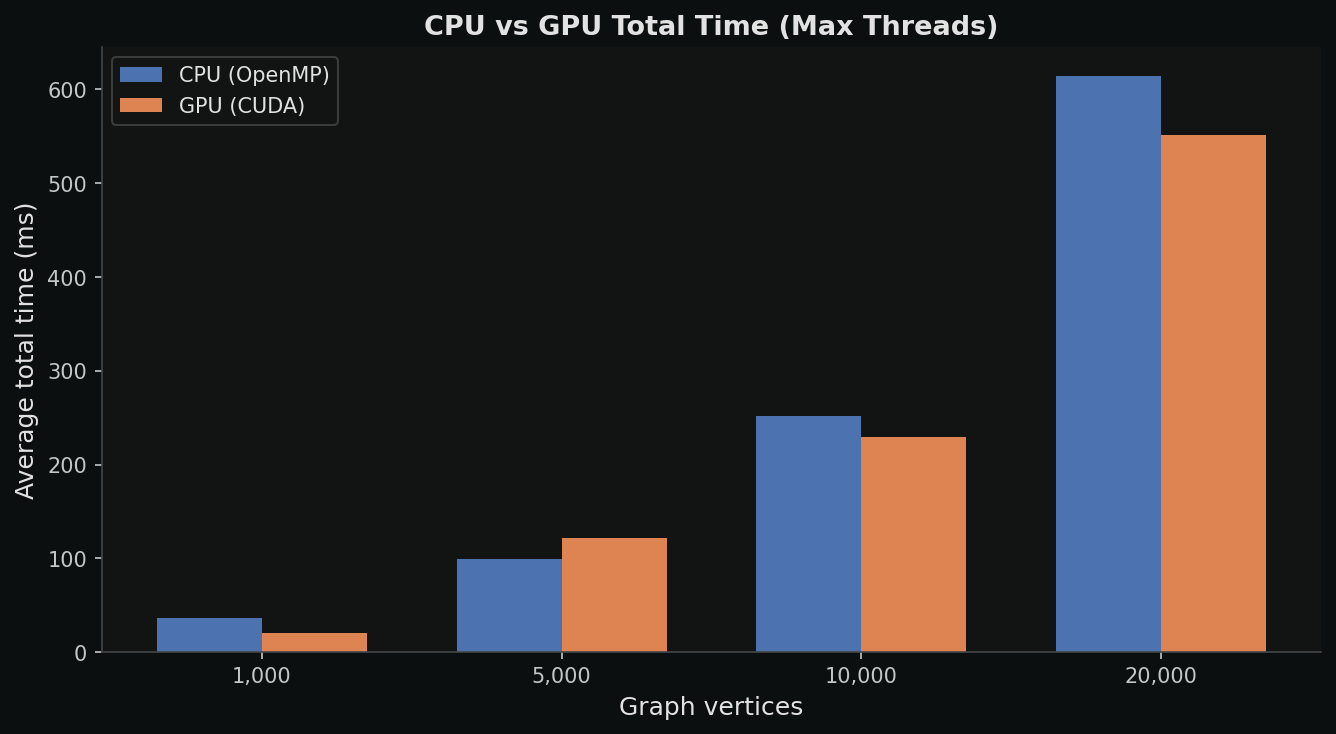
\includegraphics[width=0.9\linewidth]{cpu_gpu_total_time.png}
\caption{CPU vs GPU total time (max thread configuration). GPU shows a clear advantage for some sizes, but CPU remains competitive on medium graphs.}
\end{figure}

\begin{figure}[H]
\centering
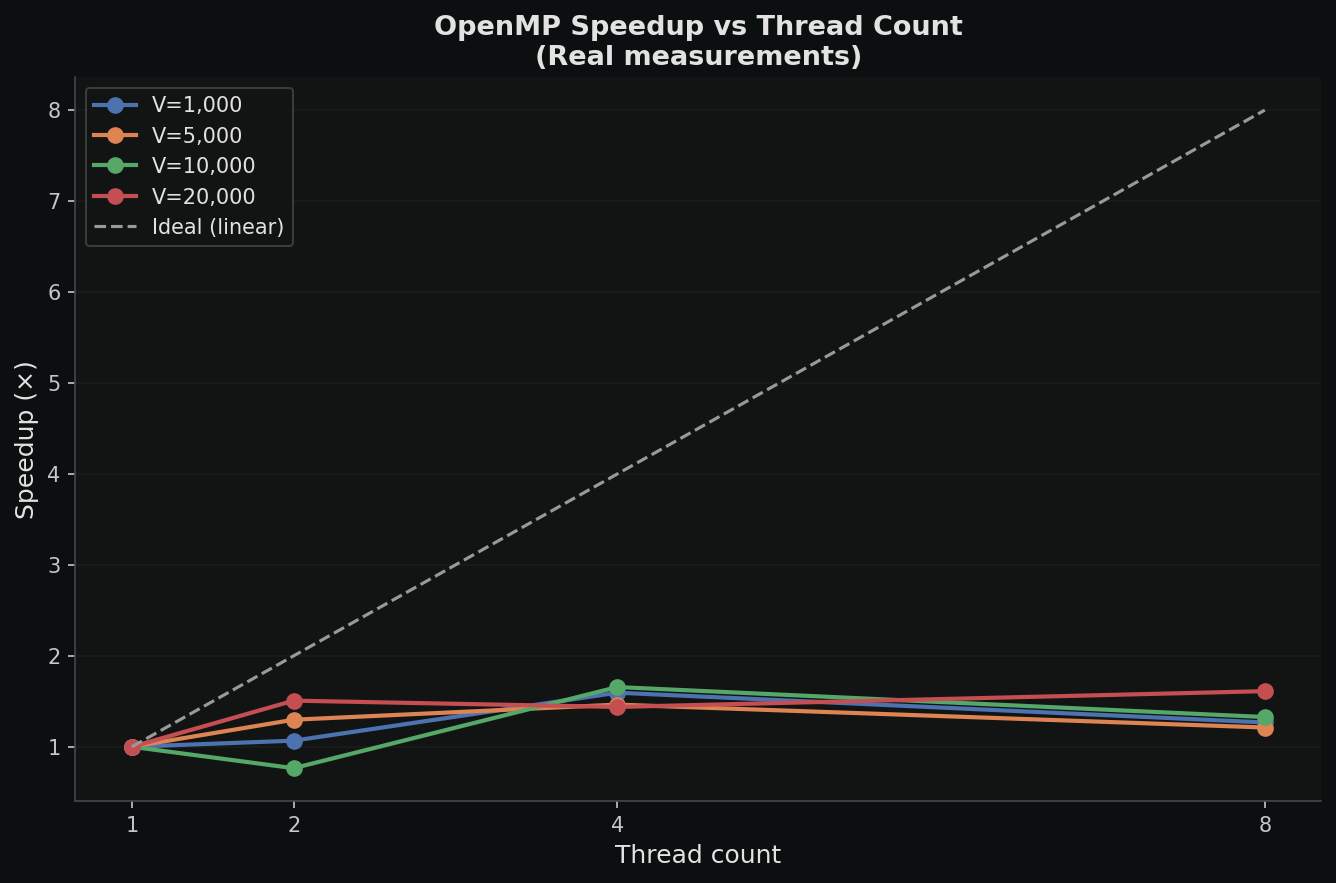
\includegraphics[width=0.9\linewidth]{speedup_curve.png}
\caption{Speedup curve from OpenMP benchmark runs. The gap from ideal linear speedup reflects synchronization overhead and memory limits.}
\end{figure}

\begin{figure}[H]
\centering
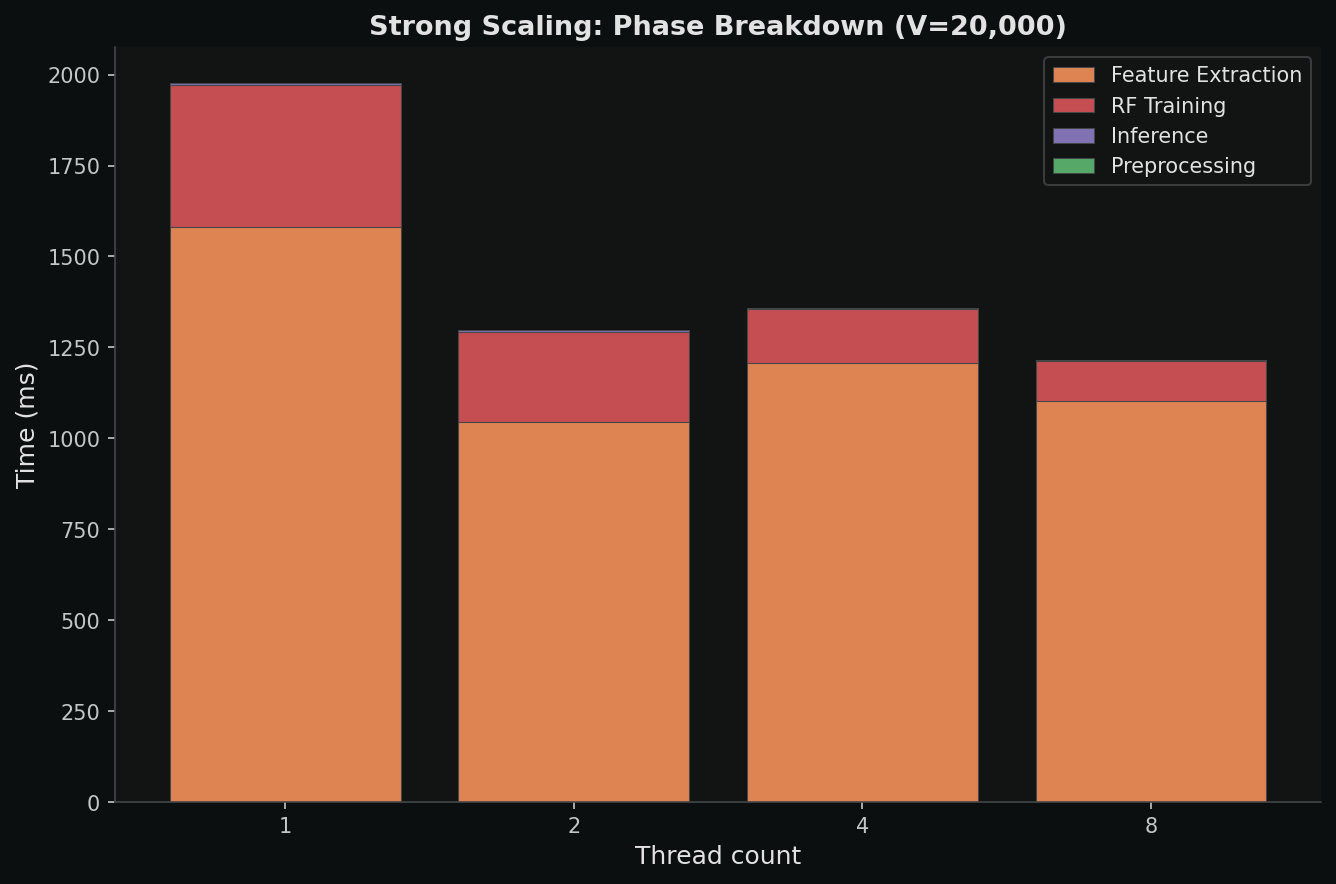
\includegraphics[width=0.9\linewidth]{strong_scaling.png}
\caption{Strong scaling phase breakdown for the largest synthetic graph size. Feature extraction and training dominate runtime at higher thread counts.}
\end{figure}

\begin{figure}[H]
\centering
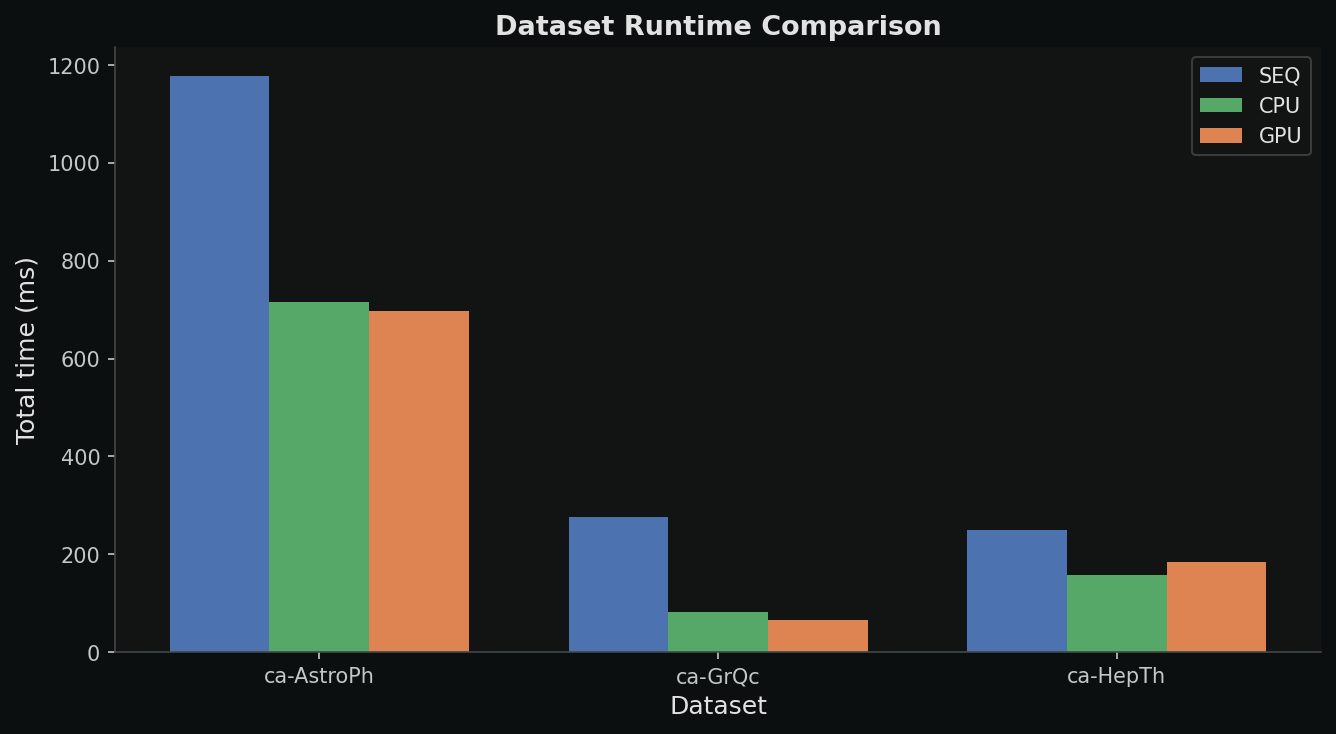
\includegraphics[width=0.9\linewidth]{dataset_runtime.png}
\caption{Dataset runtime comparison for sequential, CPU, and GPU modes. The GPU gain varies with graph density and size.}
\end{figure}

\section{Testing and Validation}
The backend includes unit tests for the CSR builder, feature extractors, and ML components. Tests run with CTest and do not require external frameworks. The test suite checks:
\begin{itemize}
  \item Correct CSR sizes and degree counts on synthetic graphs.
  \item Feature extractor correctness on small graphs where expected values are known.
  \item Random Forest accuracy on synthetic linear data.
  \item Evaluator accuracy and confusion matrix structure.
\end{itemize}

Scripts such as \texttt{perf\_smoke.sh} provide a quick sanity check for the pipeline output and the presence of the final \texttt{[RESULT]} line. This is useful for fast validation before running long benchmarks.

\section{Known Issues and Risks}
\begin{itemize}
  \item The dashboard labels the engine as GPU if a CUDA binary exists, even when runtime CUDA is unavailable and the backend falls back to CPU. This can misreport execution mode and should be checked during demos.
  \item The adaptive workload splitter assumes a non-empty graph. Empty or comment-only input files can trigger invalid sampling and should be validated before execution.
  \item The Barabasi--Albert generator does not guard against very small \texttt{--vertices} values and can create more vertices than requested. A small guard can improve robustness.
  \item Benchmark scripts do not automatically copy outputs into the \texttt{backend/plots/presentation} folder, so the dashboard can display stale results unless files are moved manually.
  \item The frontend depends on CDN assets for Tailwind and Chart.js, which can fail in offline environments.
\end{itemize}

\section{Conclusion}
GraphPulse demonstrates a complete workflow for graph analytics and classification, covering data ingestion, feature extraction, preprocessing, and parallel ML training. The system is structured cleanly, with a compact API and dashboard for interactive use. Benchmark results show meaningful speedups from OpenMP and potential benefits from GPU preprocessing, while also highlighting cases where overhead can limit gains.

The current implementation is functional and ready for classroom demonstration. Future improvements could include stronger input validation, automatic plot updates after benchmarks, and clearer GPU/CPU mode reporting in the UI.

\section*{Submission}
Submitted by:
\begin{itemize}
  \item Arpan Goyal
  \item Nitin Gupta
\end{itemize}

To: Dr. Saif Nalband

\end{document}
